They way that the CPU communicates with the GPU is with commands.
This can for instance be memory transfers and kernel launches.
These commands are sent via streams, either implicitly or explicitly.
A stream is a virtual work queue (where the operations are executed in otder) used for asynchronous operations so that the CPU can operate concurrently with the GPU.
It is possible to have multiple streams and there can be a lot of reasons and benefits for this.
It is possible to perform memory copies concurrently with kernel executions.
To support this, the "copy engine" can perform a DMA transfer on the PCI-e bus while the SM's are executing a kernel.
Kernel launches are per definition asynchronous, but memory transfers can be either synchronous or asynchronous.
To make a memory transfer asynchronous, a different set of \cuda{} functions must be used (suffixed with a "Async").
An example of asynchronous kernel launches and memory transfers can be seen in \autoref{lst:stream-default-usage}.
As all the operations are asynchronous, they will simply be executed in the order, but the CPU will not wait for the operations to finish.
In this example no specific streams are linked to the operation, which means that all operations are linked to the default stream (number zero).
\begin{lstlisting}[language=C++,caption={Default stream usage},label=lst:stream-default-usage]
int main(int argc, char ** argv) {
	cudaMemcpyAsync( ... );
	example_kernel1<<< ... >>>
	cudaMemcpyAsync( ... )
	example_kernel2<<< ... >>> }
\end{lstlisting}
If one would like to use different streams, can be de declared and used as seen in \autoref{lst:stream-cre-des}.
From here, the entire life-cycle of a \cuda{} stream can be seen.
The stream is simply used by passing the \cuda{} struct to the async memory transfer function and the kernel launch.
\begin{lstlisting}[language=C++,caption={Stream creation, usage and destruction},label=lst:stream-cre-des]
int main(int argc, char ** argv) {
	cudaStream_t stream;
	cudaStreamCreate(&stream);
	cudaMemcpyAsync(d_in, h_in, 10 * sizeof(unsigned int), cudaMemcpyHostToDevice, stream);
	example_kernel<<<10, 1024, 0, stream>>>(d_in, 10)
	cudaStreamDestroy(stream) }
\end{lstlisting}
Using streams are for instance beneficial if you have to perform computations on a large amount of data that are bigger than the GPU memory.
There are different ways to do this, where two scenarios are described below and visualized in \autoref{fig:streams-advantage}.
\begin{enumerate}
	\item[\textbf{Scenario 1}]
		\begin{enumerate}
			\item Splitting the data into smaller chunks that fit in GPU memory
			\item Copy chunk from CPU to GPU
			\item Process data
			\item Copy processed data back to the CPU
		\end{enumerate}
	\item[\textbf{Scenario 2}]
			\begin{enumerate}
				\item Splitting the data into chunks half the size of scenario 1
				\item Copy chunk from CPU to GPU to fill half of GPU memory
				\item Process data and concurrently copy new chuck of data to GPU (GPU memory is now full)
				\item Copy processed data back to the CPU and concurrently copy new chuck to GPU (replacement of the processed data)
		\end{enumerate}
\end{enumerate}
\begin{figure}[ht]
	\centering
	\fbox{
		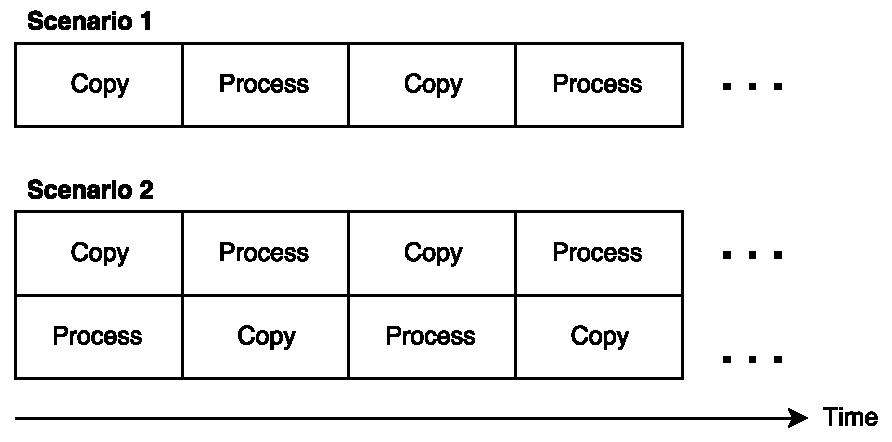
\includegraphics[width=0.5\textwidth]{figs/programming-model/streams.pdf}
	}
	\caption{Advantage of using streams}
	\label{fig:streams-advantage}
\end{figure}
To sum up, it can generally be be advantageous to use stream to overlap memory and computation and help fill GPU with smaller kernels.
%caveats --> streams and events